\chapter{INTRODUCTION}
\label{ch:introduction}
\section{Motivation and Background}
\subsection{Why Object Search Matters in AR and VR}
Finding the relevant object is often a prerequisite for doing something useful with an augmented or virtual environment. Before following an instruction, inspecting a component, or interacting with task content, a user must connect the system's intended referent with something they can see. Binetti et al. motivate AR visual-search assistance through maintenance, repair, instruction, and training, where a person must locate a real or virtual target in the surrounding scene~\cite{binetti2021outofview}. These application examples explain why search is worth supporting: assistance can help bridge the gap between knowing which item a task concerns and locating that item among competing objects.

Object search also provides a concrete task through which assistance can be studied. Zhang et al. operationalize it as finding a specified book among other books using a head-mounted AR interface~\cite{zhang2023seehear}. Their task brings together an intended target, distractors, and a search environment without requiring an entire industrial workflow. This makes it a useful precedent for investigating guidance, although finding a book is not evidence that the same interface will improve maintenance or training. The practical motivation and the scope of the evaluation must remain distinct.

In VR, the corresponding challenge is often directing attention without taking away the user's freedom to explore. HiveFive motivates guidance through the possibility of missing relevant content while looking elsewhere, including in cinematic VR, games, and collaboration~\cite{lange2020hivefive}. This is broader than object retrieval, but it shares the problem of bringing a system-relevant location into the user's attention. Kwok et al. similarly motivate gaze guidance through large search spaces and the example of locating an object described by an audio guide~\cite{kwok2022twostep}. These works justify studying the connection between a cue and its intended referent, rather than assuming that presenting information guarantees that the user will find it.

AR and VR therefore offer related but different reasons to study guided search. AR can connect instructions to the surrounding physical workspace; VR can distribute relevant content throughout a simulated environment. In either case, a cue must help the user orient and identify what matters. The present project uses passthrough mixed reality with surrounding virtual objects as a controlled setting for this interaction. Its intended contribution concerns how people receive assistance, with potential relevance to these wider applications rather than a claim of demonstrated transfer to them.

\subsection{Why the Guiding Voice Matters}
Once assistance is spoken, its usefulness depends on more than the direction encoded in the words. ``Look to your right'' describes an action, but it is also delivered by a voice the listener may welcome, recognize, or find uncomfortable. Research on gaze-contingent auditory feedback and staged guidance establishes precedents for adapting assistance to the search process~\cite{losing2014guiding,kwok2022twostep}. The question pursued here concerns the voice carrying that assistance: would directions feel or function differently if they sounded like the person receiving them?

Self-similar voice is a specific form of personalization. It uses recorded speech to synthesize a voice resembling the participant, whereas catalog personalization lets that participant choose an existing voice. Prior studies connect voice self-similarity with selected engagement and identification outcomes in a game, and with both favorable impressions and eeriness in virtual collaboration~\cite{kao2021selfsimilar,guo2024doppelganger}. These findings make self-similar assistance worth investigating without implying that it is necessarily preferable. A familiar-sounding voice could be welcome in one role and distracting in another; this study asks about the role of a spatial guide.

For designers, the useful question is consequently whether self-similar synthesis offers value beyond a voice the user already likes. Follow My Voice compares a self-similar synthetic voice with a participant-preferred catalog voice, not an intentionally poor or impersonal baseline. If participants find their clone more useful or comfortable, that would support considering resemblance as a design option in this task. If the preferred voice is easier to follow, or if resemblance introduces discomfort, that would be equally relevant to voice selection. No such outcome is assumed in advance.

Usefulness will be evaluated through both behavior and experience. Recognizing the clone is a manipulation check, not a performance benefit; liking it without searching faster is still an experience result. Likewise, completing efficiently while finding the voice eerie would distinguish task effectiveness from acceptability. The thesis therefore examines completion time, workload, motivation, and agent experience separately, rather than treating a faster or more familiar voice as universally better.

\subsection{A Controlled Setting for Self-Similar Assistance}
Follow My Voice studies this comparison in a surrounding object-search task. A seated participant wears a mixed-reality headset and views colored geometric objects distributed across eight vertical planes. The application knows which object is the target, while the participant is not given its color or shape at the start. Spoken directions first guide orientation toward the relevant wall and then refine the search within it. The participant aims a right-controller ray and presses the trigger to select the inferred target; gaze itself does not select an object.

This initially unnamed target gives the voice an ongoing instructional role. Instead of supplementing a target description that the participant can follow independently, the guidance progressively establishes which object is intended. The controlled shapes and surrounding layout make starting geometry and trial events easier to specify across the two voice conditions. They also limit the claim: this is an experiment about receiving personalized spatial assistance, not a simulation of every demand in a repair, training, or everyday retrieval task.

The central comparison holds the assistance mechanism shared while changing the assigned voice. Gaze contingency and constrained agent decisions provide the means for delivering relevant instructions; they are not additional participant treatments. This organization lets the thesis ask whether hearing guidance in one's own synthetic voice changes the efficiency or experience of being guided, while retaining the practical object-search problem that makes those instructions consequential.

\section{Problem Statement}
The central research problem is whether a self-similar synthetic voice changes task performance or the experience of assistance relative to a participant-preferred catalog voice. Answering it requires a comparison in which guidance policy, target-selection mechanics, and intended difficulty distribution remain shared. Reliable adaptive speech is therefore an experimental requirement: its directions must remain appropriate while the participant's gaze and controller move. A direction that was correct when requested can become obsolete before playback. A controller may already point at the target while an older downward correction is still waiting to speak. These failures can influence both search time and perceived responsiveness, thereby contaminating a voice comparison.

Gaze measurements also require careful interpretation. A ray intersecting an object is an observation made by the interaction system; it does not establish that the participant fixated, recognized, or understood the object. Likewise, a nearby-gaze region is a deliberate interface tolerance that may improve usability but cannot substitute for measuring spatial accuracy. Nor does a headset's nominal output rate demonstrate that the application receives distinct gaze observations at that rate~\cite{dunn2024reporting,niehorster2026dataquality}.

The thesis addresses these problems by separating observed evidence, guidance state, model decisions, and delivered speech, and it carries the same distinctions into the analysis. An instruction selected by a model is not counted as spoken until playback starts. A qualified gaze acknowledgment is distinct from a controller acknowledgment, and a controller acknowledgment does not constitute a successful trial until the trigger selection is correct. This separation is necessary both to implement responsive guidance and to explain what the participant actually experienced.

\section{Research Objectives and Questions}
The primary objective is to evaluate self-similar voice as a form of task assistance, using a participant-preferred catalog voice as the comparison within a shared gaze-contingent system. The primary research question is: will active search-completion time differ between self-similar and preferred catalog voices after accounting for absolute starting angle and repeated observations within participants? The contrast is two-sided because the current design does not justify assuming a performance advantage for self-similarity.

Secondary questions concern perceived workload and activity experience. Will the two voices differ on the six workload dimensions and their complete unweighted mean? Will they differ on interest/enjoyment, effort/importance, pressure/tension, or value/usefulness? Because these outcomes concern different constructs, the analysis will preserve those distinctions rather than pool them into a broad satisfaction score.

Exploratory questions concern agent perception, reliance, and the relationship between task difficulty and voice experience. Participants may describe a voice as more responsive or humanlike, may rely on guidance more often, or may experience a cloned voice as familiar or eerie. Such reports will be treated as judgments about an interaction, not as evidence that the system possesses intelligence, emotions, awareness, or an inner voice.

A supporting validation requirement is to make the assistance process inspectable so that technical faults do not masquerade as effects of self-similar voice. Can recorded state and speech history explain why a cue was eligible, why it played or was suppressed, and how long it waited? Can evaluation distinguish a genuinely unhelpful instruction from an acceptable alternative wording? These questions concern system validity and readiness; they support the empirical study but do not replace it.


\subsection{Research-Question Traceability}
The questions are assigned stable identifiers so that the completed results and conclusion can answer the same questions introduced here. RQ1 is the primary empirical contrast; RQ2 concerns secondary experience measures; RQ3 is exploratory. EQ1 identifies an engineering question rather than a fourth participant research question. Table~\ref{tab:rq-map} connects each question to its evidence and analysis. The identifiers organize the existing plan and do not add a new experimental factor or a directional hypothesis.

\begin{table}[htbp]\centering
\caption[Research questions and evidence requirements]{Research-question traceability for the proposed study. No empirical answer is available in this first pass.}
\label{tab:rq-map}
\small\begin{tabularx}{\linewidth}{@{}p{0.12\linewidth}p{0.39\linewidth}X@{}}\toprule
Question & Intended contrast & Evidence and reporting destination \\\midrule
RQ1 & Does self-similar voice change active completion time relative to a preferred catalog voice? & Trial timing and starting geometry; analysis in Chapter~\ref{ch:analysis}, results in Chapter~\ref{ch:evaluation}. \\
RQ2 & Do self-similar and preferred catalog voices differ in workload or motivation? & Paired block-referenced workload and separate IMI subscales; final retrospective administration. \\
RQ3 & How do voices differ in agent perception, voice experience, reliance, and search behavior? & Custom ratings, agent constructs, debrief, and valid search measures; exploratory voice-by-angle comparison. \\
EQ1 & Can the recorded sequence explain eligibility, delivery, and unhelpful guidance? & State, request, and actual playback records; supporting evaluation in Appendix~\ref{app:guidance-support}. \\\bottomrule
\end{tabularx}
\end{table}

The voice-similarity manipulation check will be reported before the outcome contrasts to aid interpretation across questions. It is not an individual exclusion gate. RQ3 includes appealing, eerie, and familiar voice experiences and the exploratory variation of the voice contrast with starting angle.

\section{Scope of the Comparison}
The independent variable is voice condition: participant-preferred catalog voice versus self-similar synthetic voice. Both conditions use gaze contingency, the same semantic phrase library, the same local geometry rules, and the same controller-selection mechanics. Consequently, the study will not isolate the benefit of gaze contingency, short-term memory, the cloud decision agent, or synthetic speech in general. Those are shared system properties.

The task is deliberately narrower than unrestricted navigation. Participants remain seated and rotate their head and chair to search surrounding planes. Guidance such as ``turn left'' concerns orientation within this setup; it does not ask them to walk toward a target. Objects are virtual, the physical room is visible through passthrough, and the target is initially unnamed. Conclusions will therefore be bounded to guided search under these conditions.

The use of one practice trial in the first assigned voice is a current protocol decision. It introduces an exposure asymmetry: whichever voice appears first also appears during practice. Counterbalancing distributes that asymmetry across voices, but does not remove learning or carryover. The analysis must retain period and assigned order, and the report must describe the practice assignment explicitly.

Figure~\ref{fig:comparison-framework} separates the voice manipulation from the shared task. A difference between conditions would require evidence from the planned study; the diagram specifies the comparison rather than predicting its direction.

\begin{figure}[htbp]
\centering
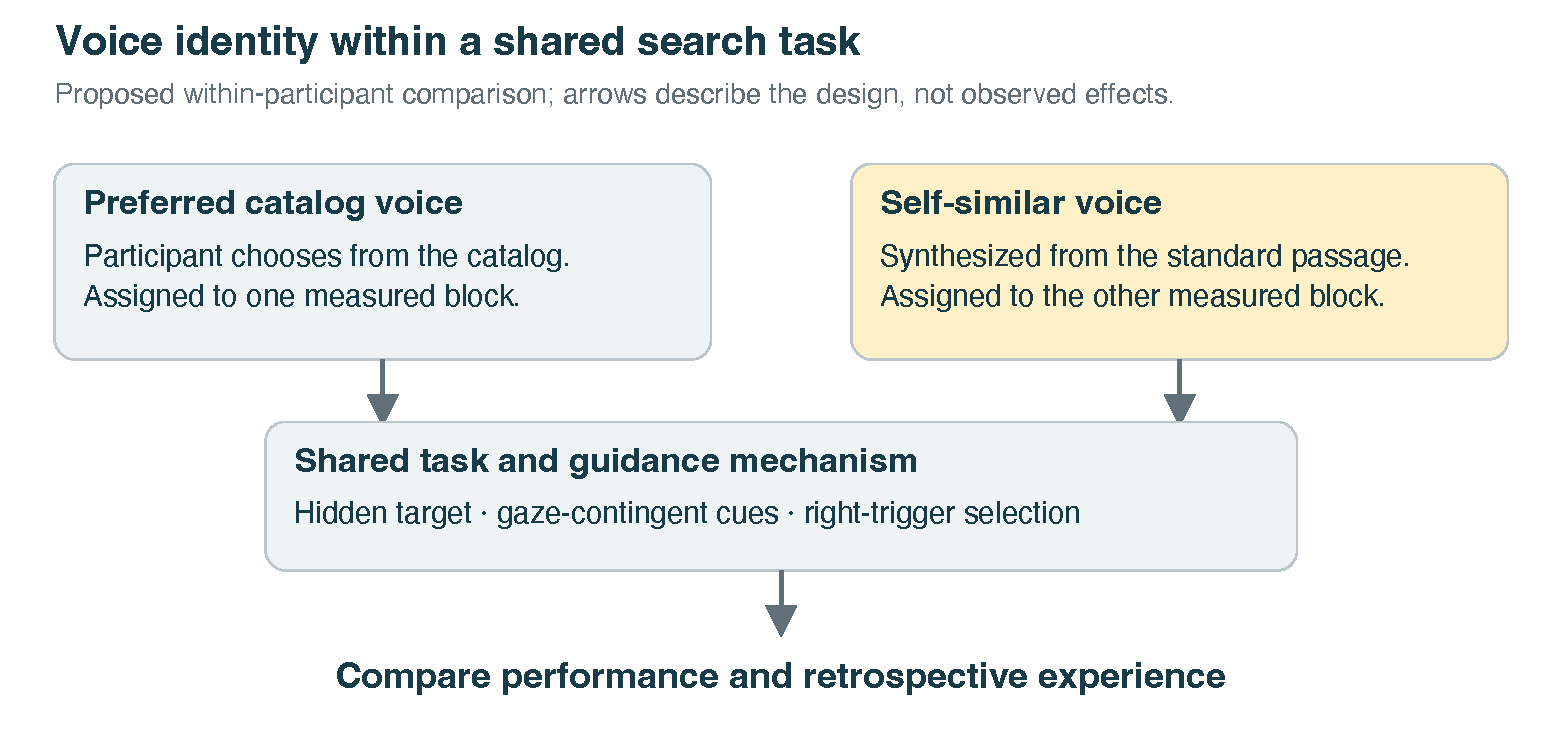
\includegraphics[width=\linewidth,alt={Two voice conditions feed a shared hidden-target search task and a paired outcome comparison.}]{figures/comparison-framework.pdf}
\caption[Voice comparison within the shared search task]{Proposed comparison of preferred and self-similar voices within a shared task and guidance mechanism. The schematic identifies the intended manipulation and outcome families; it does not depict observed effects.}
\label{fig:comparison-framework}
\end{figure}


\section{Contributions of This First Pass}
The thesis develops an empirical comparison of self-similar voice with a preferred alternative in mixed-reality task assistance. Its conceptual contribution is to distinguish resemblance from preference and to examine performance alongside the favorable or uncomfortable experience of hearing one's own synthetic voice. The study will not assume that greater perceived similarity implies faster search, lower workload, or a more welcome agent.

The methodological contribution is a within-participant design that makes this comparison operational: two counterbalanced voice blocks, a shared hidden-target task, explicit trigger selection, comparable starting-difficulty allocations, retrospective voice-referenced questionnaires, and a planned repeated-measures analysis. Manipulation checks and acoustic-quality reporting will help establish what the voice conditions actually delivered before their outcomes are interpreted.

The implemented guidance and recording platform supports that empirical contribution. Local spatial eligibility, constrained agent decisions, prepared speech, and synchronized review make it possible to inspect what each participant heard and whether delivery problems affected the comparison. The platform is the apparatus for studying self-similar voice; a provider benchmark or a new gaze-guidance algorithm is not the thesis's primary claim.

The empirical contribution remains pending. This draft does not report a recruited sample, condition means, significance tests, or participant quotations. A completed thesis will replace the pending results sections with the frozen study's actual voice-condition outcomes and revise its abstract and conclusion accordingly.

\section{Organization of the Thesis}
Chapter~\ref{ch:literature} establishes the voice rationale; Chapters~\ref{ch:system} and~\ref{ch:methodology} describe the apparatus and comparison. Chapters~\ref{ch:measurement}--\ref{ch:analysis} define measurement and analysis, and Chapter~\ref{ch:evaluation} organizes the pending results. The discussion and conclusion address self-similar assistance and its limits. Appendices retain instruments, data definitions, readiness decisions, and implementation details.
